\documentclass{standalone}
\usepackage{pgfplots}
\pgfplotsset{compat=newest}

\pagestyle{empty}

\begin{document}
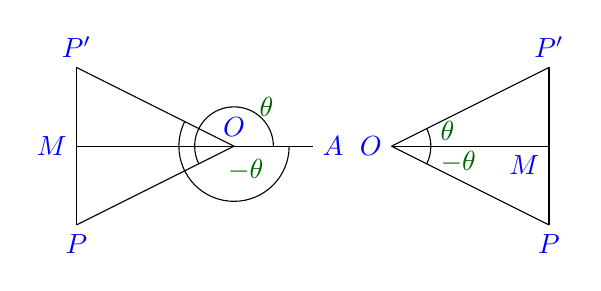
\begin{tikzpicture}

\draw (2, -3) -- (3, -3);
\draw (2, -3) -- (0, -3);
\draw (2, -3) -- (0, -2);
\draw (0, -3) -- (0, -2);
\draw [blue] (3, -3) node[anchor=west] {$A$};
\draw [blue] (2, -3) node[anchor=south] {$O$};
\draw [blue] (0, -3) node[anchor=east] {$M$};
\draw [blue] (0, -2) node[anchor=south] {$P'$};
\draw [black!60!green] (2.2, -2.5) node[anchor=west] {$\theta$};
\draw (2.5, -3) arc[start angle=0, end angle=207, radius=0.5];
\draw (2, -3) -- (0, -4);
\draw (0, -3) -- (0, -4);
\draw [blue] (0, -4) node[anchor=north] {$P$};
\draw (2.7, -3) arc[start angle=360, end angle=153, radius=0.7];
\draw [black!60!green] (1.8, -3.3) node[anchor=west] {$-\theta$};

\draw (4, -3) -- (6, -3);
\draw (4, -3) -- (6, -2);
\draw (6, -3) -- (6, -2);
\draw [blue] (4, -3) node[anchor=east] {$O$};
\draw [blue] (6, -3) node[anchor=north east] {$M$};
\draw [blue] (6, -2) node[anchor=south] {$P'$};
\draw [black!60!green] (4.5, -2.8) node[anchor=west] {$\theta$};
\draw (4.5, -3) arc[start angle=0, end angle=27, radius=0.5];
\draw (4, -3) -- (6, -4);
\draw (6, -3) -- (6, -4);
\draw [blue] (6, -4) node[anchor=north] {$P$};
\draw (4.5, -3) arc[start angle=360, end angle=333, radius=0.5];
\draw [black!60!green] (4.5, -3.2) node[anchor=west] {$-\theta$};

\end{tikzpicture}
\end{document}
